\documentclass[fullscreen=true, bookmarks=false]{beamer}
\usepackage[utf8]{inputenc}
\usepackage[main = russian, english]{babel}

\usetheme{Boadilla}
\usepackage[cp1251]{inputenc}
\usepackage{xcolor}

\usepackage{amsmath,amsfonts,amssymb,amsthm,mathtools}
\usepackage{wasysym, dsfont, dashrule}

\usepackage{float, wrapfig, subcaption}

\usepackage{multirow, multicol}
\usepackage{enumerate}
\usepackage[shortlabels]{enumitem}
\usepackage{cancel}

\usepackage{epigraph}
\usepackage{physics}
\usepackage{indentfirst}
\usepackage{subfiles}
\date{}

\begin{document}

\begin{frame}
\begin{center} 
{\LARGE {\bf Anti-Dyson limit shape}}
\end{center}\\

\begin{center}
{\large { докладчики: Садреев Амир, Сенчуков Лев, Cуспицын Константин}}\\

\end{center}
\end{frame}

\begin{frame}
{\bf Диаграммы Юнга}
\begin{figure}
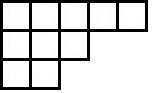
\includegraphics[width=0.4\linewidth]{young_diagram_1.jpg}\\
\end{figure}
\begin{center}
\begin{*equation}
    10 = 5 + 3 + 2
\end{*equation}
\end{center}
Число разбиений для заданного числа $n$:
\begin{equation}
    p \propto  e^{c\sqrt{n}}
\end{equation}
\begin{center}
\begin{*equation}
    p(5) = 7
\end{*equation}
\begin{*equation}
    p(20) = 627
\end{*equation}
\begin{*equation}
    p(100) \approx 190 \cdot 10^{6}
\end{*equation}
\end{center}
\end{frame}
\begin{frame}
{\bf Случаная диаграмма Юнга}
{\bf Простейший случай}

Можно ввести вероятностную меру на множестве диаграмм Юнга

Рассмотри простейший случай:
\begin{equation}
    \mu_\lambda = q^{\abs{\lambda}}
\end{equation}
Для такой меры можно вычислить статсумму:
\begin{equation}
    \mathcal{Z} = \prod_{n = 0}^{\infty}\frac{1}{1 - q^{n}}
\end{equation}
\end{frame}
\begin{frame}
{\bf Предельная форма}
    Введем переменные $x$ и $y$, а таже параметр $h$ такой, что  $q = e^{-h}$
\begin{figure}
\label{wrap-fig:1}
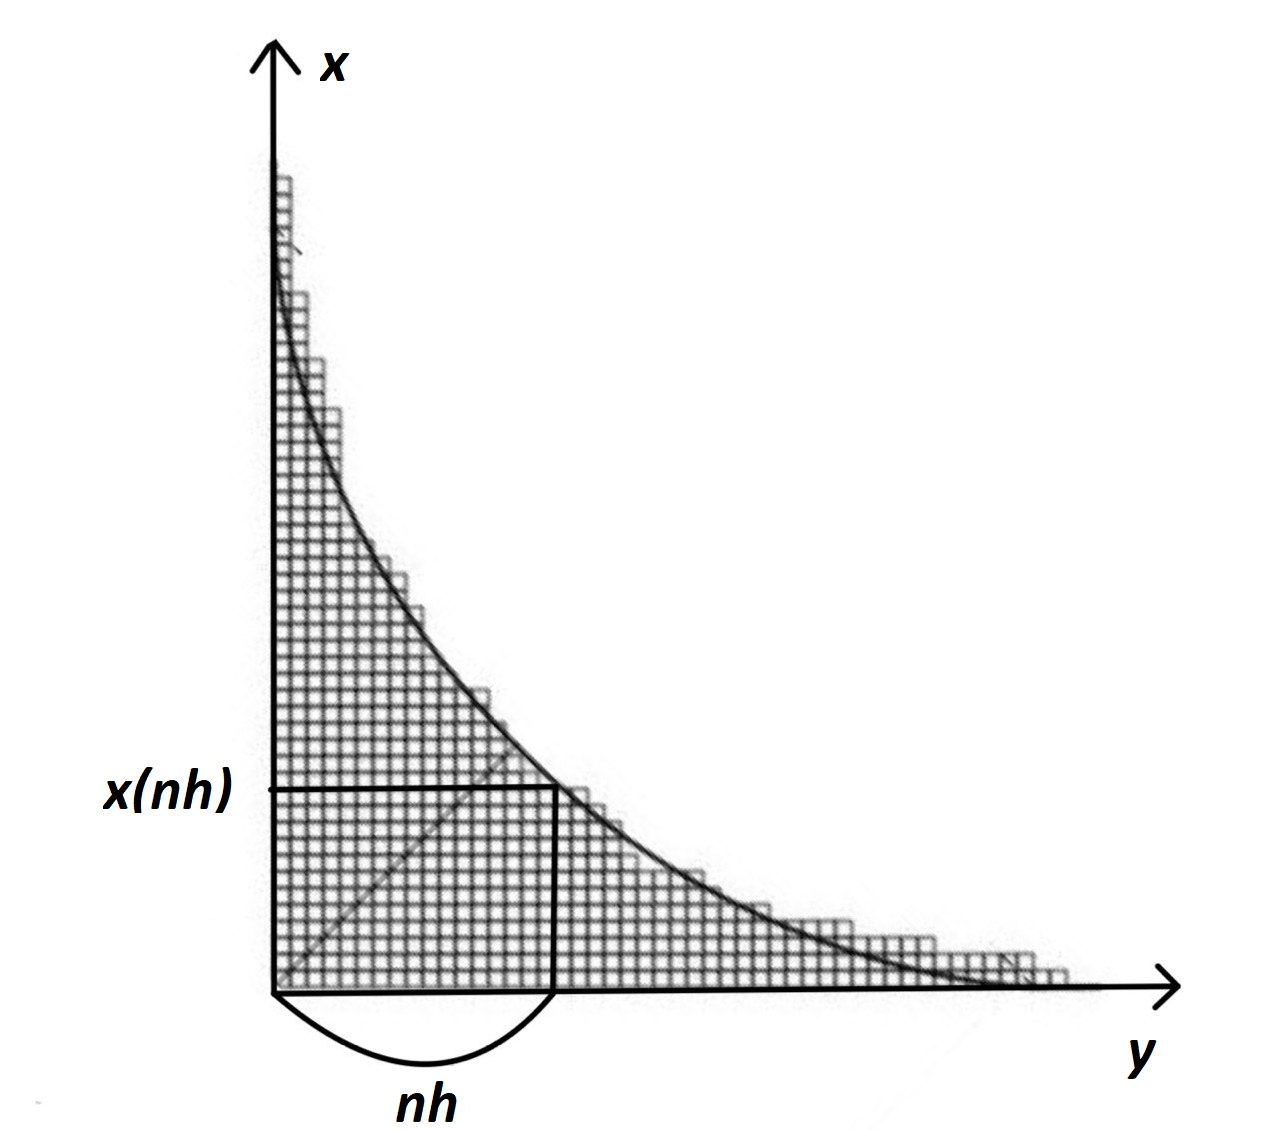
\includegraphics[width=6.5cm]{young_diagram_3.jpg}
\end{figure} 
\end{frame}
\begin{frame}
В пределе $h \rightarrow 0$ Возникает предельная форма $x(y)$.
\begin{equation}
    e^{-x} + e^{-y} = 1
\end{equation}
Такая кривая, что 
\begin{equation}
    \langle (x - x(y))^{2}\rangle = h^{2}\sum_{\ell = 0}^{\infty}\frac{\ell e^{-\ell y}}{1 - e^{-\ell h}} \rightarrow 0
\end{equation}
\end{frame}
\begin{frame}
{\bf Случайная диаграмма Юнга}
{\bf Модифицированная мера}
В некоторых теориях возникает другое выражение для $\mu_{\lambda}$:
\begin{equation}
    \mu_{\lambda} = \prod_{(i,j) \in \lambda}q\frac{((\ell + 1)\varepsilon_1 - a\varepsilon_2 + \varepsilon_3)(-\ell\varepsilon_1 + (a + 1)\varepsilon_2 + \varepsilon_3)}{((\ell + 1)\varepsilon_1 - a\varepsilon_2)(-\ell\varepsilon_1 + (a + 1)\varepsilon_2)}
\end{equation}
\begin{center}
\begin{*equation}
    \varepsilon_1, \varepsilon_2 \in \mathbb{C}
\end{*equation}
\end{center}
\begin{figure}
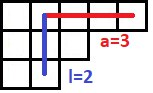
\includegraphics[width=0.4\linewidth]{young_diagram_2.jpg}\\
\end{figure}
\end{frame}

\begin{frame}
{\bf Предельные случаи}
Можно также рассмотреть различные предельные случаи данной меры:
\\
1) Мера Планшереля
\begin{center}
\begin{*equation}
    q \rightarrow 0, \quad \varepsilon_{3} \rightarrow \infty, \quad q\varepsilon_3^2 = \Lambda^{2}
\end{*equation}
\end{center}
\begin{equation}
\mu_{\lambda} = \prod_{(i,j) \in \lambda} \frac{-\Lambda^2}{((\ell + 1)\varepsilon_1 - a\varepsilon_2)(-\ell\varepsilon_1 + (a + 1)\varepsilon_2)}
\end{equation}
2) Равномерная мера
\begin{center}
\begin{*equation}
    \varepsilon_{3} \rightarrow 0
\end{*equation}
\end{center}
\begin{equation}
    \mu_{\lambda} = q^{\abs{\lambda}}
\end{equation}
\end{frame}

\begin{frame}
{\bf Y наблюдаемая}
Введем наблюдаемые:
\begin{equation}
    c_{ij} = \varepsilon_1(i-1)-\varepsilon_2(j-1)
\end{equation}
\begin{equation}
    C(x)=\prod_{(i,j)\in\lambda}(x - c_{ij})
\end{equation}
\begin{equation}
    Y(x)|_\lambda=x\frac{C(x-\varepsilon_1)C(x-\varepsilon_2)}{C(x)C(x-\varepsilon_1-\varepsilon_2)}
\end{equation}
$Y(x)$ можно переписать в ином виде
\begin{equation}
    Y(x)|_\lambda = \frac{\prod_{\square \in \partial_{+}\lambda}(x - c_\square)}{\prod_{\blacksquare \in \partial_{-}\lambda}(x - c_{\blacksquare})}
\end{equation}
\begin{figure}
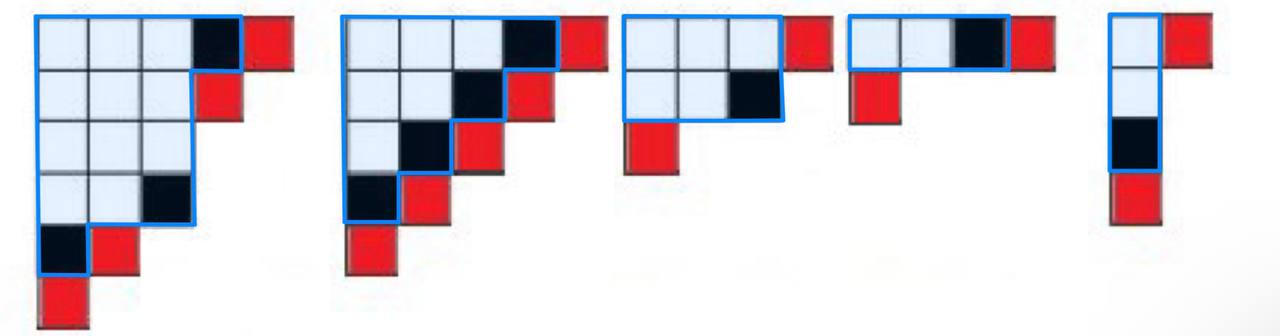
\includegraphics[width=0.8\linewidth]{young_diagram_4.jpg}\\
\end{figure}
\end{frame}

\begin{frame}
{\bf $qq$ - характер}
Рассмотрим коррелятор
$
    \langle Y(x + \varepsilon_{1} + \varepsilon_{2}) + \frac{\Lambda^2}{Y(x)} \rangle
$    с мерой \newline

$    \mu_{\lambda} = \prod_{(i,j) \in \lambda} \frac{\Lambda^2}{((\ell + 1)\varepsilon_1 - a\varepsilon_2)(-\ell\varepsilon_1 + (a + 1)\varepsilon_2)}$.
Оказывается, такой коррелятор \newline

не имеет полюсов.
\begin{equation}
    Y(x) = x + O(1), x \rightarrow \infty
\end{equation}
\begin{equation}
\langle Y(x + \varepsilon_{1} + \varepsilon_{2}) + \frac{\Lambda^2}{Y(x)} \rangle = (x + \varepsilon_1 + \varepsilon_2)\mathcal{Z}
\end{equation}
Отсюда получаем уравнения Швингера-Дайсона:
\begin{equation}
    0 = \varepsilon_1 \varepsilon_2 \langle \abs{\lambda} \rangle + \Lambda \langle 1 \rangle
\end{equation} 
\begin{equation}
    0=\varepsilon_1 \varepsilon_2\frac{\Lambda }{2}\frac{d}{d\Lambda}\mathcal{Z}+\Lambda^2\mathcal{Z} \quad \mathcal{Z}=e^{-\frac{\Lambda^2}{\varepsilon_1 \varepsilon_2}}
\end{equation}
\end{frame}

\begin{frame}
{Предельная форма}
\begin{equation}
    y(x) = \langle \langle Y(x) \rangle \rangle
\end{equation}
В пределе 
\begin{equation}
    \varepsilon_1, \varepsilon_2 \rightarrow 0
\end{equation}
\begin{equation}
    y + \frac{\Lambda^2}{y} = x  \quad y = \frac{1}{2}(x + \sqrt{x^2 - 4\Lambda^2})
\end{equation}
Предельная форма может быть найдена из уравнения 
\begin{equation}
    y(x) = exp(\frac{1}{2} \int_{-\infty}^{+\infty} f''(t)log(x - t)dt)
\end{equation}
\begin{equation}
    f''(x) = \frac{2}{\pi\sqrt{4\Lambda^2 - x^2}}
\end{equation}
\end{frame}
\begin{frame}
\begin{figure}
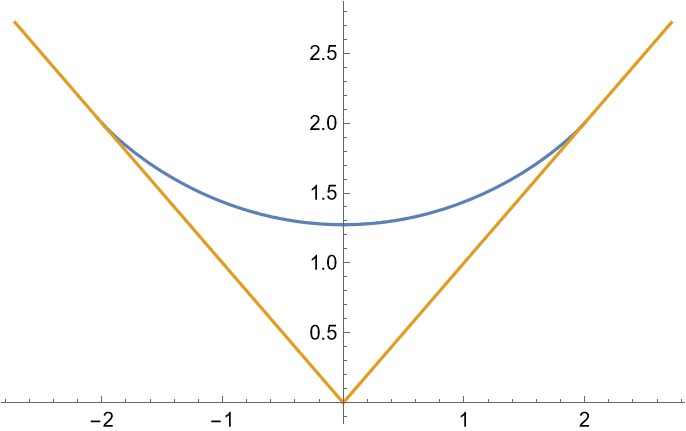
\includegraphics[width=0.55\linewidth]{young_diagram_5.jpg}\\
\end{figure}
\begin{figure}
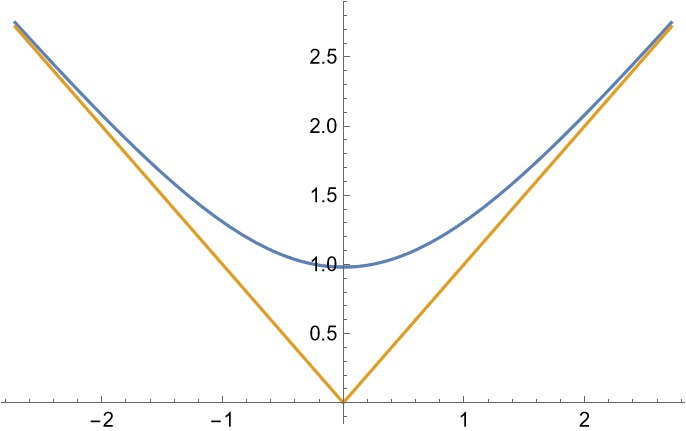
\includegraphics[width=0.55\linewidth]{young_diagram_7.jpg}\\
\end{figure}
\end{frame}
\begin{frame}
    {\bf Y(x) для равномерной меры}
    случай $\varepsilon_1 = -\varepsilon_2$
    \begin{equation}
    f(t) = \sqrt{2}log(2cosh(\frac{t}{\sqrt{2}}
    ))
\end{equation}
\begin{equation}
    y(x) = exp(\frac{1}{2}\int_{-\infty}^{+\infty}f''(t)log(x - \sqrt{2}t\varepsilon_1))
\end{equation}
\begin{equation}
    y(x) = \frac{i\pi\varepsilon_1}{2}exp(\frac{i\pi}{2\varepsilon_1} x-\frac{i}{\pi}\psi(\frac{1}{2}+\frac{x}{2i\pi\varepsilon_1})-\gamma(\frac{i}{\pi}+1)-\frac{2i}{\pi}log(2))
\end{equation}
\begin{figure}
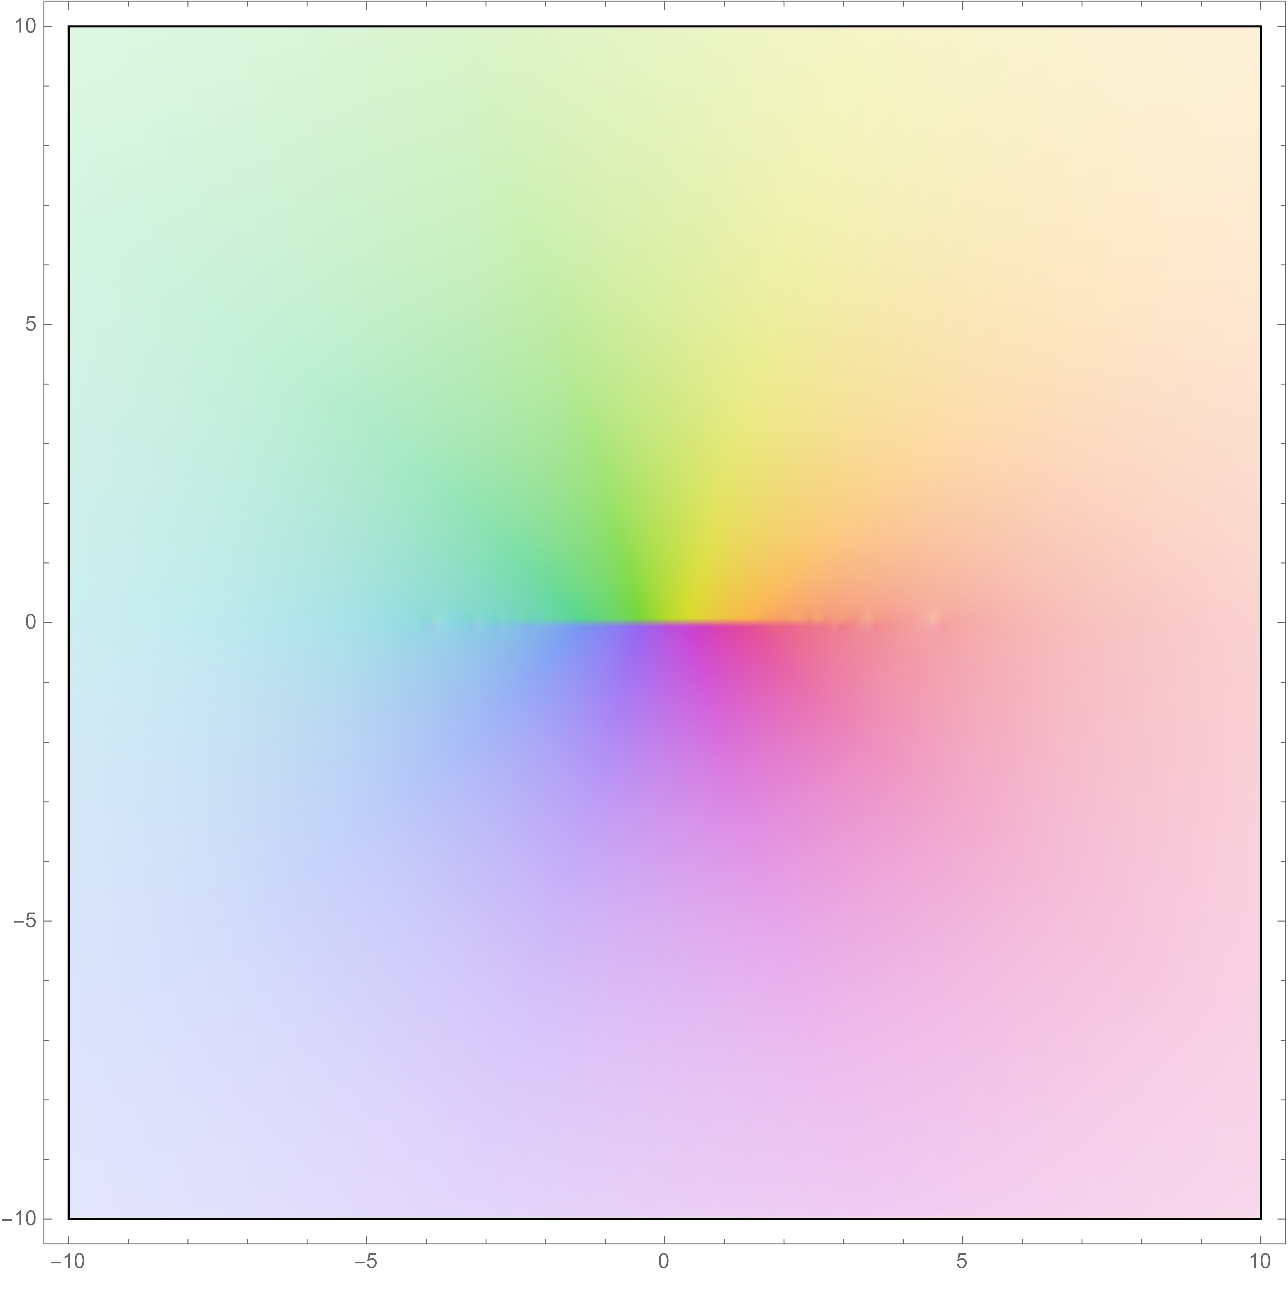
\includegraphics[width=0.35\linewidth]{young_diagram_6.pdf}\\
\end{figure}
\end{frame}
\begin{frame}
{\bf Что еще можно сделать?}
\begin{enumerate}
\item[1)] Рассмотрение в случае меры более общего вида ($\varepsilon_1 \neq -\varepsilon_2$, произвольный $\varepsilon_{3}$)
\item[2)] Исследование физических приложений (четырехмерные суперсимметричные калибровочные теории, теория струн)
\end{enumerate}
\end{frame}


\end{document}

